\documentclass[../main.tex]{subfiles}

\begin{document}
\section{线性模型}
线性模型一般形式

$$f(x)=w_{1}x_{1}+w_{2}x_{2}+\cdots+w_{d}x_{d}+b$$

$x=(x_{1};x_{2};\ldots;x_{d})$是由属性描述的示例，其中$x_{i}$是$x$在第$i$个属性上的取值

向量形式
$$
f(x)=w^{\mathrm{T}}x+b$$

其中$w=(w_{1};w_{2};\ldots;w_{d})$

\subsection{线性回归（linear regression）}
\begin{enumerate}
    \item \textbf{线性回归目的：}学得一个线性模型，以尽可能准确地预测实值输出标记。

    \item \textbf{离散属性处理：}
    \begin{itemize}
        \item \textbf{有“序”关系：}连续化为连续值。
        \item \textbf{无“序”关系：}若有 $k$ 个属性值，则转化为 $k$ 维向量。
        \item \textbf{例：}
        \begin{itemize}
            \item 尺码“\text{小 / 中 / 大}”有序，可转化为 $1,2,3$；
            \item 颜色“\text{红 / 绿 / 蓝}”无序，可转化为 $(1,0,0),(0,1,0),(0,0,1)$。
        \end{itemize}
    \end{itemize}
    \textcolor{red}{本节下面的小写楷体东西看个乐呵得了，考这个我吃}
    {\small\kaishu
    \item \textbf{单变量线性回归：}
    \begin{itemize}
        \item 给定数据集$D = \{(\mathbf{x}_1, y_1), (\mathbf{x}_2, y_2), \dots, (\mathbf{x}_m, y_m)\}$，其中$\mathbf{x}_i = (x_{i1}; x_{i2}; \dots; x_{id}), y_i \in \mathbb{R}$
        \item \textbf{模型：}
        $$
        f(x)=wx+b
        $$
        
        \item \textbf{参数/模型估计：}最小二乘法
        $$
        \begin{aligned}
        (w^{*},b^{*})
        &=\underset{(w,b)}{\operatorname*{argmin}}\sum_{i=1}^{m}(f(x_{i})-y_{i})^{2} \\
        &=\underset{(w,b)}{\operatorname*{argmin}}\sum_{i=1}^{m}(y_{i}-wx_{i}-b)^{2}
        \end{aligned}
        $$
        
        \item \textbf{平方误差：}
        $$
        E_{(w,b)}=\sum_{i=1}^{m}(y_i-wx_i-b)^2
        $$
        
        \item \textbf{闭式解：}
        $$
        w=\frac{\sum_{i=1}^{m} y_i(x_i-\bar{x})}{\sum_{i=1}^{m} x_i^2-\frac{1}{m}\left(\sum_{i=1}^{m}x_i\right)^2}
        $$
        $$
        b=\frac{1}{m}\sum_{i=1}^{m}(y_i-wx_i)
        $$
        其中
        $$
        \bar{x}=\frac{1}{m}\sum_{i=1}^{m}x_i
        $$
    \end{itemize}

    \item \textbf{多元线性回归：}
    \begin{itemize}
        \item \textbf{给定数据集：}
        $$
        D=\{(\mathbf{x}_1,y_1),(\mathbf{x}_2,y_2),\cdots,(\mathbf{x}_m,y_m)\}
        $$
        其中
        $$
        \mathbf{x}_i=(x_{i1};x_{i2};\cdots;x_{id}),\qquad y_i\in\mathbb{R}
        $$
        
        \item \textbf{多元线性回归目标：}
        $$
        f(\mathbf{x}_i)=\mathbf{w}^{\mathrm{T}}\mathbf{x}_i+b
        $$
        使得
        $$
        f(\mathbf{x}_i)\simeq y_i
        $$
        
        \item \textbf{向量化表示：}把 $\mathbf{w}$ 和 $b$ 吸收入向量形式
        $$
        \hat{\mathbf{w}}=(\mathbf{w};b)
        $$
        数据集表示为
        $$
        \mathbf{X}=
        \begin{pmatrix}
        x_{11} & x_{12} & \cdots & x_{1d} & 1 \\
        x_{21} & x_{22} & \cdots & x_{2d} & 1 \\
        \vdots & \vdots & \ddots & \vdots & \vdots \\
        x_{m1} & x_{m2} & \cdots & x_{md} & 1
        \end{pmatrix},
        \qquad
        \mathbf{y}=
        \begin{pmatrix}
        y_1\\
        y_2\\
        \vdots\\
        y_m
        \end{pmatrix}
        $$
        
        \item \textbf{最小二乘法：}
        $$
        \hat{\mathbf{w}}^{*}
        =\underset{\hat{\mathbf{w}}}{\operatorname*{argmin}}
        (\mathbf{y}-\mathbf{X}\hat{\mathbf{w}})^{\mathrm{T}}(\mathbf{y}-\mathbf{X}\hat{\mathbf{w}})
        $$
        
        令
        $$
        E_{\hat{\mathbf{w}}}=(\mathbf{y}-\mathbf{X}\hat{\mathbf{w}})^{\mathrm{T}}(\mathbf{y}-\mathbf{X}\hat{\mathbf{w}})
        $$
        对 $\hat{\mathbf{w}}$ 求导得到
        $$
        \frac{\partial E_{\hat{\mathbf{w}}}}{\partial \hat{\mathbf{w}}}
        =2\mathbf{X}^{\mathrm{T}}(\mathbf{X}\hat{\mathbf{w}}-\mathbf{y})
        $$
        
        \item \textbf{正则方程：}
        $$
        \mathbf{X}^{\mathrm{T}}\mathbf{X}\hat{\mathbf{w}}=\mathbf{X}^{\mathrm{T}}\mathbf{y}
        $$
        
        \item \textbf{满秩时闭式解：}若 $\mathbf{X}^{\mathrm{T}}\mathbf{X}$ 是满秩矩阵或正定矩阵，则
        $$
        \hat{\mathbf{w}}^{*}=(\mathbf{X}^{\mathrm{T}}\mathbf{X})^{-1}\mathbf{X}^{\mathrm{T}}\mathbf{y}
        $$
        
        \item \textbf{对应模型：}
        $$
        f(\hat{\mathbf{x}}_i)=\hat{\mathbf{x}}_i^{\mathrm{T}}(\mathbf{X}^{\mathrm{T}}\mathbf{X})^{-1}\mathbf{X}^{\mathrm{T}}\mathbf{y}
        $$
        
        \item \textbf{梯度下降：}当 $\mathbf{X}^{\mathrm{T}}\mathbf{X}$ 不是满秩矩阵，或样本量极大、特征极多时，求解正则方程计算代价高昂甚至不可行，此时可采用梯度下降。
        \begin{itemize}
            \item 初始化参数 $\mathbf{w}$（如全零）；
            \item 重复执行直至收敛：
            $$
            w_j:=w_j-\alpha\frac{\partial J(\mathbf{w})}{\partial w_j}
            $$
            对所有的 $j$ 同时更新，其中 $\alpha$ 是学习率。
        \end{itemize}
    \end{itemize}

    \item \textbf{广义线性模型：}
    \begin{itemize}
        \item \textbf{一般形式：}
        $$
        y=g^{-1}(\mathbf{w}^{\mathrm{T}}\mathbf{x}+b)
        $$
        
        \item \textbf{联系函数（link function）：}
        $$
        g(\cdot)
        $$
        称为联系函数，通常为单调可微函数。
        
        \item \textbf{特例：}对数线性回归是 $g(\cdot)=\ln(\cdot)$ 时广义线性模型的特例。
    \end{itemize}
        \item \textbf{补充：对数线性回归、岭回归与 Lasso 回归}
\begin{itemize}
    \item 补充：
    \begin{itemize}
        \item 对数线性回归：是广义线性模型在线性回归中的一个特例；
        \item 岭回归、Lasso 回归：是在普通多元线性回归基础上加入正则化项得到的改进模型。
    \end{itemize}
    \item \textbf{三者对比：}
    
    \begin{center}
    \renewcommand{\arraystretch}{1.35}
    \begin{tabularx}{\textwidth}{>{\raggedright\arraybackslash}p{2.2cm}
                                  >{\raggedright\arraybackslash}X
                                  >{\raggedright\arraybackslash}p{4.2cm}
                                  >{\raggedright\arraybackslash}p{2.8cm}}
    \toprule
    方法 & 基本形式 / 目标函数 & 重要特点 & 典型作用 \\
    \midrule
    对数线性回归 &
    $\ln y=\mathbf{w}^{\mathrm T}\mathbf{x}+b$；
    等价于 $y=e^{\mathbf{w}^{\mathrm T}\mathbf{x}+b}$ &
    对输出标记取对数后再做线性建模；属于广义线性模型，联系函数为 $g(\cdot)=\ln(\cdot)$ &
    适用于输出与输入呈指数关系的情形 \\
    
    岭回归（Ridge） &
    $\displaystyle
    \min_{\mathbf{w}}
    \|\mathbf{Xw}-\mathbf{y}\|_2^2+\lambda\|\mathbf{w}\|_2^2
    $ &
    加入 $L_2$ 正则项；会压缩系数，但通常不会把系数压到 $0$；$\lambda$ 越大，收缩越强 &
    缓解过拟合；减弱多重共线性影响；保留全部特征 \\
    
    Lasso 回归 &
    $\displaystyle
    \min_{\mathbf{w}}
    \frac{1}{2n_{\mathrm{samples}}}\|\mathbf{Xw}-\mathbf{y}\|_2^2+\lambda\|\mathbf{w}\|_1
    $ &
    加入 $L_1$ 正则项；不仅压缩系数，还可能将部分系数直接压为 $0$ &
    缓解过拟合；可进行特征选择；适合高维稀疏情形 \\
    \bottomrule
    \end{tabularx}
    \end{center}

    \item \textbf{岭回归补充：}
    \begin{itemize}
        \item $\lambda\ge 0$ 是控制系数收缩量的复杂性参数；
        \item 当 $\lambda=0$ 时，退化为普通线性回归；
        \item 当 $\lambda\to +\infty$ 时，参数趋近于 $0$；
        \item $\lambda$ 的确定可用岭迹分析或 $K$ 折交叉验证。
    \end{itemize}

    \item \textbf{岭回归与 Lasso 回归区别：}
    \begin{itemize}
        \item 岭回归：所有特征通常都被保留，只是系数被缩小；
        \item Lasso 回归：部分不重要特征的系数可直接变为 $0$，从而实现特征选择。
    \end{itemize}
\end{itemize}
    }

\end{enumerate}





\subsection{线性分类}
线性回归直接做分类问题\footnote{分类本质上是要在数据点之间找到一个决策边界，因此在线性回归基础上引入一个非线性映射函数（激活函数）映射为我们想要的输出，比如类别或概率}：（1）输出值范围不匹配（2）对异常值敏感
\begin{enumerate}
    \item \textbf{对数几率回归}
    \begin{itemize}
        \item \textbf{模型定义}：对数几率回归是一种用于\textbf{二元分类}的线性模型。它通过构造广义线性回归函数，并使用sigmoid函数将回归值映射到$(0,1)$之间的概率值。
        \item \textbf{极大似然法}：最大化对数似然函数
    \end{itemize}
    
    \item \textbf{softmax回归}
    \begin{itemize}
        \item \textbf{模型目标}：逻辑回归的扩展，用于\textbf{多分类}问题。它通过softmax函数将线性输出映射为多个类别的概率分布。
        \item \textbf{softmax函数}：
        $$
        P(y=k\mid x)=\frac{e^{w_k^{\mathrm T}x+b_k}}{\sum_{j=1}^{K}e^{w_j^{\mathrm T}x+b_j}},\qquad k=1,2,\dots,K
        $$
    \end{itemize}    
    
    \item \textbf{感知机}
    \begin{itemize}
        \item \textbf{统一模型：}
        $$
        y=
        \begin{cases}
        1, & w_1x_1+w_2x_2+b\ge 0 \\
        0, & w_1x_1+w_2x_2+b<0
        \end{cases}
        $$
        \item \textbf{应用举例：}相同的感知机结构，不同的参数配置，可以实现多种逻辑门功能。
        {\small\kaishu
        \begin{itemize}
            \item \textbf{与门（AND）：}
            $$
            w_1=0.5,\quad w_2=0.5,\quad b=-0.7
            $$
            决策边界：
            $$
            0.5x_1+0.5x_2-0.7\ge 0
            $$
            
            \item \textbf{或门（OR）：}
            $$
            w_1=0.5,\quad w_2=0.5,\quad b=-0.2
            $$
            决策边界：
            $$
            0.5x_1+0.5x_2-0.2\ge 0
            $$
            
            \item \textbf{与非门（NAND）：}
            $$
            w_1=-0.5,\quad w_2=-0.5,\quad b=0.7
            $$
            决策边界：
            $$
            -0.5x_1-0.5x_2+0.7\ge 0
            $$
        \end{itemize}
        }
    \end{itemize}
\end{enumerate}

\subsection{线性判别分析（LDA）}
\begin{figure}[H]
    \centering
    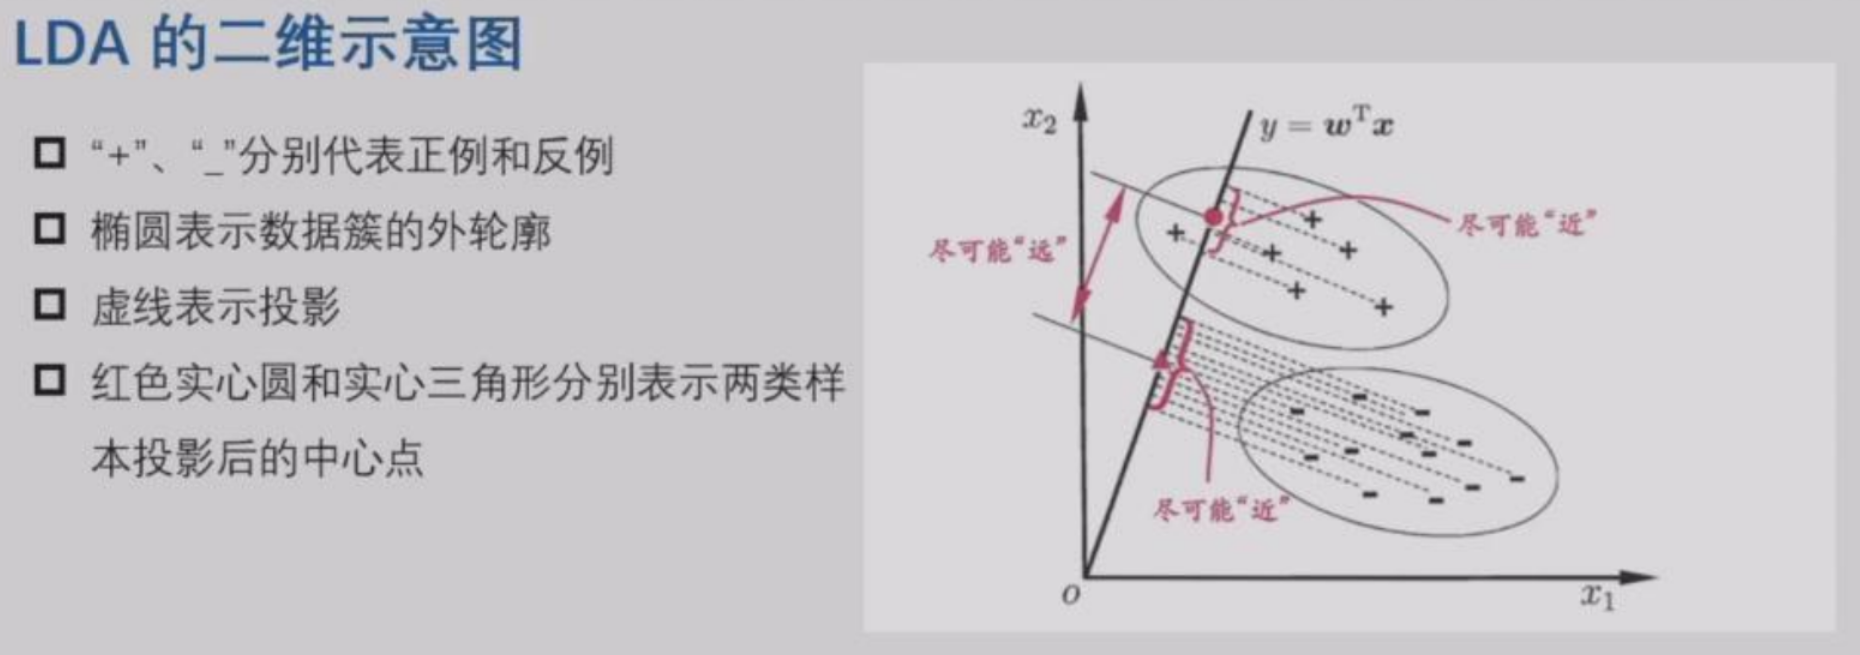
\includegraphics[width=0.75\linewidth]{images/LDA.png}
    \caption{LDA的二维示意图}
    \label{fig:placeholder}
\end{figure}

\begin{enumerate}
    \item \textbf{基本思想：}LDA 需要寻找一条合适的直线
    $$
    y=\mathbf{w}^{\mathrm T}\mathbf{x}
    $$
    使得数据集中的样例投影到该直线后，同类样例的投影点尽可能接近，不同类样例的投影点尽可能远离。

    \item \textbf{分类方法：}对新样例，先将其投影到该直线上，再根据投影点的位置判断样本类别。

    \item \textbf{贝叶斯决策论解释：}当两类数据先验相同、满足高斯分布且协方差矩阵相等时，LDA 可达到最优分类。

    \item \textbf{多分类扩展：}LDA 可以扩展到多分类学习。多分类 LDA 将样本投影到 $d'$ 维空间，且通常
    $$
    d'\ll d
    $$
    因此 LDA 也可视为一种监督降维技术。

    \item \textbf{多分类学习拆分策略：}
    \begin{itemize}
        \item \textbf{一对一（One vs. One, OvO）}
        \item \textbf{一对其余（One vs. Rest, OvR）}
        \item \textbf{多对多（Many vs. Many, MvM）}
    \end{itemize}
\end{enumerate}
\subsection{关键问题扩展}
\begin{enumerate}
    \item \textbf{过拟合阶数选择}
    \begin{enumerate}
        \item 欠拟合问题根本原因是特征维度过少，导致拟合函数无法较好刻画训练集，训练误差较大；可通过增加特征维度来解决。
        \item 过拟合问题根本原因是特征维度过多，导致拟合函数过度适应训练集而对新数据预测较差；可通过减少特征维度、正则化、数据集扩增等方法解决。
    \end{enumerate}

    \item \textbf{基函数扩展}
    \begin{enumerate}
        \item \textbf{动机：}
        \begin{itemize}
            \item 线性模型本质上对应线性决策边界；
            \item 现实问题常需要非线性建模；
        \end{itemize}

        \item \textbf{解决方法：}可通过基函数将原始特征空间映射到更高维空间，再在新空间中用线性模型拟合非线性关系。
        
        \item \textbf{一般形式：}
        $$
        y(x)=w_0+\sum_{j=1}^{M}w_j\phi_j(x)
        $$
        其中：
        \begin{itemize}
            \item $\phi_j(x)$：第 $j$ 个基函数（非线性变换）；
            \item $M$：基函数数量，决定模型复杂度。
        \end{itemize}

        \item \textbf{作用：}
        \begin{itemize}
            \item 用基函数 $\phi(x)$ 替换输入变量 $x$；
            \item 将线性拟合形式扩展为固定非线性函数的线性组合。
        \end{itemize}

        \item \textbf{优点：}
        \begin{itemize}
            \item \textbf{提升模型表达能力}：把原始输入映射到更高维或更合适的特征空间后，原本复杂的非线性关系可能在新空间里变成线性可表示，提升拟合效果。

            \item \textbf{保持优化简单}：虽然模型对输入是非线性的，但对参数 w 仍然是线性的，因此仍可使用线性模型成熟的求解方法。
        \end{itemize}

        \item \textbf{缺点：}
        \begin{itemize}
            \item \textbf{过拟合}：基函数过多时，模型可能把噪声也拟合进去。

            \item \textbf{计算开销增加}：特征维度变高，训练和预测成本都上升。

            \item \textbf{泛化能力下降}：训练误差下降，但测试误差可能上升。
        \end{itemize}

        \item \textbf{常见基函数类型：}多项式基函数、高斯径向基（RBF）、Sigmoid基函数、傅里叶基函数。
    \end{enumerate}
    \item \textbf{类别不平衡处理}
    没发ppt，前面都是智云的，我力竭了。
\end{enumerate}
\end{document}